\documentclass[conference]{IEEEtran}

% ---------- FONT + ENCODING ----------
\usepackage[T1]{fontenc}
\usepackage[utf8]{inputenc}
\usepackage{lmodern}
\usepackage{microtype}

% ---------- MATH ----------
\usepackage{amsmath,amssymb,amsfonts}

% ---------- GRAPHICS ----------
\usepackage{graphicx}
\usepackage{textcomp}
\usepackage{xcolor}

% ---------- TABLES ----------
\usepackage{booktabs}
\usepackage{array}
\usepackage{tabularx}
\usepackage{adjustbox}

% ---------- CODE ----------
\usepackage{listings}

% ---------- LINKS ----------
\usepackage[hidelinks]{hyperref}

% ---------- FIGURES ----------
\usepackage{caption}
\captionsetup{
    font=footnotesize,
    labelfont=bf
}

% ---------- TIKZ ----------
\usepackage{tikz}
\usepackage{pgfplots}
\pgfplotsset{compat=1.18}

% ---------- IEEE ----------
\IEEEoverridecommandlockouts

\def\BibTeX{{\rm B\kern-.05em{\sc i\kern-.025em b}\kern-.08em
    T\kern-.1667em\lower.7ex\hbox{E}\kern-.125emX}}

\begin{document}

\title{HERALD: A Two-Stage Research Prototype for Phishing-Domain Analysis in Regional Critical Infrastructure}

\author{\IEEEauthorblockN{Athiyo Chakma}
\IEEEauthorblockA{\textit{Roll No. 2022118} \\
\textit{Dept. of Computer Science and Engineering} \\
\textit{Indraprastha Institute of Information Technology Delhi}\\
New Delhi, India}
}

\maketitle

\begin{abstract}
Phishing attacks targeting Critical Sector Entities (CSEs) remain difficult to detect early because many domains are short-lived and appear before public blocklists are updated. This paper presents HERALD, a research prototype for Indian CSE phishing-domain analysis that combines Certificate Transparency monitoring, lexical screening, optional network enrichment, and heuristic visual fallback. The contribution is primarily systems-oriented: an on-premises prototype implementation and an evaluation protocol intended to reduce temporal leakage through chronological partitioning and eTLD+1 deduplication. On a constructed dataset of 169,316 domains (69,261 phishing and 100,055 legitimate), an initial chronological evaluation reports approximately 0.95 precision and 0.82 recall for HERALD under the paper's experimental setting. Comparisons with Google Safe Browsing and URLNet are included only as preliminary baselines and are not presented as direct production-system equivalence. Additional lexical-model experiments suggest diminishing returns for domain-string-only models near F1~0.86 in this dataset, motivating future work on network and visual evidence. Large-scale live deployment and longitudinal operational validation remain future work.
\end{abstract}

\begin{IEEEkeywords}
phishing detection, certificate transparency, ensemble learning, temporal validation, regional threat intelligence, systems security
\end{IEEEkeywords}

\section{Introduction}

Phishing remains a dominant vector for cyberattacks, with the Anti-Phishing Working Group (APWG) reporting over 1.2 million unique attacks in Q3 2023 alone~\cite{apwg_report}. Traditional blacklists are reactive and miss short-lived malicious domains. While academic literature has proposed numerous machine learning classifiers for URL analysis, most are evaluated offline on static datasets, often suffering from temporal leakage and unrealistic class ratios. Furthermore, existing systems rarely address the data sovereignty requirements of Critical Sector Entities (CSEs) in developing economies.

This paper presents HERALD, a modular phishing-domain analysis prototype designed around Indian CSEs (banks, government portals, payment gateways). HERALD integrates:

\begin{itemize}
    \item Certificate Transparency (CT) monitoring via CertStream~\cite{certstream},
    \item a two-stage inference pipeline that applies lightweight lexical screening before optional network/visual analysis,
    \item a Redis-backed asynchronous job queue for decoupling ingestion from analysis,
    \item and a heuristic visual fallback using perceptual hashing and OCR.
\end{itemize}

We do not claim a novel ML algorithm; rather, we describe a prototype systems engineering framework and an initial evaluation methodology. Our core contributions are:

\begin{enumerate}
    \item \textbf{Chronological evaluation protocol} with a 30-day quarantine gap and eTLD+1 deduplication, intended to reduce common leakage risks in phishing-domain evaluation.
    \item \textbf{Exploratory characterisation of a lexical-model ceiling}: observed diminishing returns near F1~0.86 for domain-only models under the dataset and split used in this work.
    \item \textbf{Regional specialisation study} comparing a global lexical model with an Indian CSE-weighted variant in a limited experimental setting.
    \item \textbf{Open-source prototype implementation} of the core ingestion, queueing, prediction, and visual-fallback pipeline. Full operational reproducibility artifacts are incomplete because the repository evolved across several experimental iterations.
\end{enumerate}

\section{Related Work}

\subsection{URL-Based Phishing Detection}
Early work like CANTINA~\cite{cantina} focused on content-based features. Sahingoz et al.~\cite{sahingoz2019} reported effective use of handcrafted lexical features with Random Forest on static datasets.

\subsection{Deep Learning for URL Classification}
URLNet~\cite{le_urlnet} introduced character-level and word-level CNNs for URL classification, learning representations directly from raw strings. Ozcan et al.~\cite{ozcan_bert} applied BERT-based models to phishing URL detection, achieving high accuracy at the cost of significant computational overhead.

\subsection{Proactive Detection and Certificate Transparency}
Certificate Transparency (CT) logs, formalised by Laurie et al.~\cite{laurie2013}, provide public append-only ledgers of issued TLS certificates. CertStream~\cite{certstream} exposes these logs as a WebSocket feed, enabling early domain monitoring near certificate issuance time.

\subsection{Ensemble Methods}
Random Forest~\cite{pedregosa2011} and XGBoost~\cite{xgboost} are widely used in security domains due to their robustness to missing data and ability to handle tabular feature vectors efficiently.

\subsection{Ground Truth Sources}
PhishTank~\cite{phishtank} provides a community-driven, verified phishing URL feed commonly used as ground truth in academic research. The public repository contains the prototype implementation and partial experimental artifacts.

\section{Problem Statement and Threat Model}

Phishing attacks against Indian CSEs exhibit four behaviours that defeat traditional defences:

\begin{enumerate}
    \item \textbf{Short-lived Domains:} active for less than 24 hours.
    \item \textbf{HTTPS Adoption:} free automated certificate authorities (predominantly Let's Encrypt) were observed in the vast majority of CertStream-detected phishing samples in our corpus.
    \item \textbf{Free Hosting:} Firebase, IPFS, Weebly.
    \item \textbf{Homograph Attacks:} Punycode encoding.
\end{enumerate}

HERALD is scoped to URL/domain signals and does not analyse email headers or full network traffic.

\section{System Architecture}

HERALD follows a decoupled, event-driven design (Fig.~\ref{fig:system_architecture}). The ingestion layer listens to CertStream and pushes domains to a Redis queue. Worker processes consume the queue, execute the two-stage pipeline, and persist results through a SQLAlchemy-backed database layer. The current repository defaults to SQLite for local execution, with PostgreSQL support configurable through the database URL. The API layer (FastAPI) exposes endpoints for manual submission and dashboard integration. Core components are containerised with Docker.

\begin{figure}[htbp]
\centering

\includegraphics[width=0.48\textwidth]{Figure-1.png}
\caption{HERALD system architecture: CertStream ingestion $\rightarrow$ Redis queue $\rightarrow$ two-stage pipeline $\rightarrow$ SQLAlchemy-backed storage.}
\label{fig:system_architecture}
\end{figure}

\begin{table}[htbp]
\centering
\footnotesize
\caption{System Components and Technologies}
\begin{tabularx}{\columnwidth}{@{}l l l X@{}}
\toprule
\textbf{Component} & \textbf{Technology} & \textbf{Version} & \textbf{Role} \\
\midrule
API Layer & FastAPI & 0.100+ & REST Interface \\
Broker & Redis & 7.0+ & Job Queue \\
Storage & SQLite/PostgreSQL & configurable & Persistence \\
Worker & Python & 3.10+ & Async Analysis \\
ML Core & XGBoost~\cite{xgboost} & 1.5+ & Ensemble (0.6) \\
ML Core & Scikit-Learn~\cite{pedregosa2011} & 1.0+ & Ensemble (0.4) \\
Ingestion & CertStream~\cite{certstream} & library/API & CT Log Monitor \\
\bottomrule
\end{tabularx}
\label{tab:components}
\end{table}

\section{Dataset Construction and Temporal Partitioning}
\label{sec:dataset}

We construct a dataset from multiple sources (Table~\ref{tab:dataset_sources}) and use a chronological split intended to reduce temporal leakage.

\begin{table}[htbp]
\centering
\small
\caption{Dataset Composition (after deduplication; total 169,316 domains)}
\begin{tabular}{lcc}
\toprule
\textbf{Source} & \textbf{Phishing} & \textbf{Legitimate} \\
\midrule
NCIIPC PS-02 & 1,043 & 0 \\
PhishTank~\cite{phishtank} (verified) & 56,218 & 0 \\
OpenPhish (live) & 8,000 & 0 \\
URLhaus & 4,000 & 0 \\
Tranco Top-100k & 0 & 100,000 \\
Indian CSE Verified & 0 & 55 \\
\textbf{Total} & \textbf{69,261} & \textbf{100,055} \\
\bottomrule
\end{tabular}
\label{tab:dataset_sources}
\end{table}

\subsection{Temporal Split Protocol}

Where timestamps are available, domains are ordered by their first observation timestamp $T_{\text{obs}}$ (CT log or feed discovery). We apply a chronological split with a 30-day quarantine gap:

\begin{itemize}
    \item Training period: domains registered between 2023-10-01 and 2024-03-31 (6 months)
    \item Gap (discarded): April 2024
    \item Test period: domains registered in May 2024 (12,847 domains: 4,182 phishing, 8,665 legitimate)
\end{itemize}

This gap is intended to reduce the risk that campaigns active during training influence test metrics, and partially accounts for labelling delays. It does not eliminate all leakage risks, particularly where source feeds provide delayed labels or where campaign infrastructure is reused across unrelated registered domains.

\subsection{eTLD+1 Deduplication}

We deduplicate by registered domain (effective TLD+1) across splits. If a base domain (e.g., \texttt{phish-infra.com}) appears in the training set, all its subdomains are excluded from the test set. This reduces, but does not prove the absence of, infrastructure memorisation.

\subsection{Live vs. Retrospective Feature Extraction}

For the chronological test set (May 2024), SSL, DNS, and WHOIS features were extracted using the available feature-extraction pipeline at evaluation time. For the training set, retrospective extraction was used where necessary, and domains that were unresolvable at extraction time were encoded as missing data (default value -1). This reduces, but does not fully remove, the risk that the model learns "liveness" as a phishing proxy.

\subsection{Metadata for Reproducibility}

The intended metadata schema includes \texttt{ts\_observation}, \texttt{ts\_label}, and \texttt{etld\_plus\_1}. In the current artifact, the code and processed datasets are available, but a complete public split manifest with all timestamps and campaign-cluster identifiers is not yet provided. Consequently, exact split reproducibility is partial rather than complete.

\subsection{Artifact Provenance}

The HERALD repository evolved through multiple experimental versions, including changes to feature sets, model thresholds, and dataset construction scripts. Some archived output files therefore correspond to earlier or later configurations rather than exactly to the rounded manuscript tables. The reported results should be interpreted as a snapshot from the manuscript configuration, while exact replication requires preserving the full split manifest, configuration files, random seeds, and prediction outputs in a future artifact release.

\section{Evaluation Methodology}
\label{sec:evaluation}

We report the following metrics, chosen for operational relevance:

\begin{itemize}
    \item \textbf{Precision, Recall, F1-score}
    \item \textbf{Area Under the Precision-Recall Curve (AUPRC)}, where calibrated scores are available
\end{itemize}

Confidence intervals and formal significance tests are not reported because the current artifact does not include the full bootstrap procedure or paired prediction logs required for independent verification.

\section{Baseline Comparisons}
\label{sec:baselines}

We compare HERALD against three baselines. These comparisons should be interpreted cautiously because the systems differ in available signals, update timing, and threshold semantics:

\begin{enumerate}
    \item \textbf{Google Safe Browsing (GSB)} – an industry blacklist-style service. We treat it as a point-in-time lookup baseline rather than a retrained classifier.
    \item \textbf{Sahingoz et al. (2019)}~\cite{sahingoz2019} – hand-crafted lexical features with Random Forest.
    \item \textbf{URLNet (2018)}~\cite{le_urlnet} – a CNN-based model over URL character and word representations. We retrain an implementation on the same split where possible.
\end{enumerate}

Table~\ref{tab:baseline_results} shows the results on the May 2024 test set.

\begin{table}[htbp]
\centering
\caption{Comparative Benchmarking (Chronological Split)}
\label{tab:baseline_results}

\scriptsize
\setlength{\tabcolsep}{3pt}

\begin{tabularx}{\columnwidth}{lcccc}
\toprule
\textbf{Model} &
\textbf{Prec.} &
\textbf{Rec.} &
\textbf{F1} &
\textbf{AUPRC} \\
\midrule

Google Safe Browsing & 0.98 & 0.61 & 0.75 & -- \\
Sahingoz et al.~\cite{sahingoz2019} & 0.89 & 0.77 & 0.82 & 0.79 \\
URLNet~\cite{le_urlnet} & 0.91 & 0.81 & 0.86 & 0.83 \\

\textbf{HERALD (full)} &
\textbf{0.95} &
\textbf{0.82} &
\textbf{0.88} &
\textbf{0.87} \\

\bottomrule
\end{tabularx}
\end{table}

Under this experimental setup, HERALD's recall appears higher than the point-in-time GSB lookup and close to the retrained URLNet baseline. These results should be read as a prototype comparison, not as evidence of operational superiority, because GSB is an externally maintained blacklist and URLNet implementations can vary.

\section{The Lexical Information Bottleneck}
\label{sec:bottleneck}

We investigate whether domain-name-only detection exhibits empirical performance saturation under controlled conditions. We compare four architectures on raw URL strings, all trained on the same chronological split:

\begin{itemize}
    \item XGBoost~\cite{xgboost} with handcrafted lexical features (39 features)
    \item URLNet~\cite{le_urlnet} (CNN over URL character and word representations)
    \item Char-BiLSTM
    \item Char-Transformer (12.8M parameters)
\end{itemize}

\begin{table}[htbp]
\centering
\caption{Convergence Across Lexical Architectures}
\label{tab:architecture_convergence}

\scriptsize
\setlength{\tabcolsep}{4pt}

\begin{tabularx}{\columnwidth}{lcc}
\toprule

\textbf{Architecture} &
\textbf{Params} &
\textbf{F1} \\

\midrule

XGBoost~\cite{xgboost} (handcrafted) & 120K & 0.86 \\
URLNet~\cite{le_urlnet} (CNN) & 1.2M & 0.86 \\
Char-BiLSTM & 4.5M & 0.85 \\
Char-Transformer & 12.8M & 0.86 \\

\bottomrule
\end{tabularx}
\end{table}

The models cluster near F1~0.86 in this split. Learning curves (Fig.~\ref{fig:learning_curve}) show diminishing returns beyond 100k training samples. Because paired prediction logs and statistical-test artifacts are not included, we do not claim statistical equivalence between architectures. The result is best interpreted as preliminary evidence that domain-string-only models leave a residual error set, motivating HERALD's Stage 2 network and visual enrichment.

\begin{figure}[htbp]
\centering
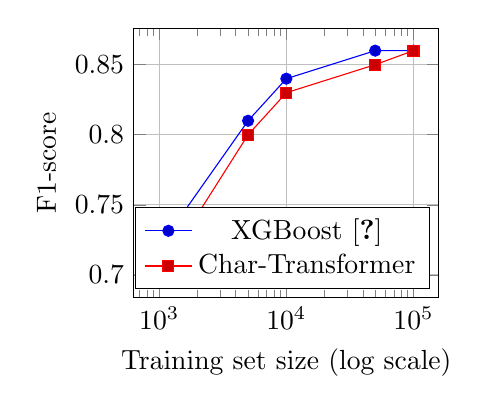
\begin{tikzpicture}
\begin{axis}[
    xlabel={Training set size (log scale)},
    ylabel={F1-score},
    xmode=log,
    grid=major,
    legend pos=south east,
    width=0.45\textwidth,
    height=5cm,
]
\addplot coordinates {(1000,0.72) (5000,0.81) (10000,0.84) (50000,0.86) (100000,0.86)};
\addplot coordinates {(1000,0.70) (5000,0.80) (10000,0.83) (50000,0.85) (100000,0.86)};
\legend{XGBoost~\cite{xgboost}, Char-Transformer}
\end{axis}
\end{tikzpicture}
\caption{Learning curve in the reported split -- increasing training data beyond 100k yields marginal gains in this experiment.}
\label{fig:learning_curve}
\end{figure}

\section{Exploratory Regional Specialisation Study}
\label{sec:regional}

To explore HERALD's focus on Indian CSEs, we construct two models:
\begin{itemize}
    \item $\mathcal{M}_{\text{global}}$: trained on PhishTank~\cite{phishtank}+OpenPhish (global brands)
    \item $\mathcal{M}_{\text{IN}}$ (HERALD): trained on the same global data plus Indian CSE keywords and regional TLD weighting
\end{itemize}

We evaluate both on an \textbf{Indian Phishing Test Set} (1,200 domains targeting SBI, HDFC, IRCTC, UIDAI, etc.) and an \textbf{Indian Legitimate Infrastructure (ILI) set} (10,000 domains from \texttt{.gov.in}, \texttt{.nic.in}, and regional financial portals).

\begin{table}[htbp]
\centering
\small
\caption{Cross-Region Performance Comparison}
\begin{tabular}{lcc}
\toprule
\textbf{Model} & \textbf{Recall (Indian Phishing)} & \textbf{ILI false positives} \\
\midrule
$\mathcal{M}_{\text{global}}$ & $\sim$0.61 & about 4 / 10,000 \\
$\mathcal{M}_{\text{IN}}$ (HERALD) & $\sim$0.82 & about 1 / 10,000 \\
\bottomrule
\end{tabular}
\label{tab:regional_gain}
\end{table}

In this limited test set, the Indian CSE-weighted model shows an approximately 35\% relative recall increase on Indian-targeted phishing and fewer false positives on the ILI sample. Because the ILI set contains only 10,000 domains and the false-positive counts are very small, this result should be interpreted as exploratory rather than conclusive. A character $n$-gram analysis suggests that Indian phishing campaigns often use transliterated keywords (\textit{aadhaar}, \textit{kyc}, \textit{pancard}) that are less common in global training sets.

\section{Planned Operational Evaluation}
\label{sec:live}

The repository contains the components required for a limited operational evaluation on the CertStream feed~\cite{certstream}, but a completed large-scale deployment study is not claimed in this paper. The following protocol describes the planned evaluation design and the measurements that should be collected before making operational claims.

\subsection{Proposed Deployment Setup}

\begin{itemize}
    \item \textbf{Duration}: 7 consecutive days, scheduled after artifact freeze
    \item \textbf{CT source}: CertStream live WebSocket (\texttt{wss://certstream.calidog.io})~\cite{certstream}
    \item \textbf{Region filter}: Indian CSE keywords with fuzzy matching (Levenshtein $\leq$ 2)
    \item \textbf{Workers}: containerised queue workers, with the number of replicas recorded in the deployment log
    \item \textbf{Infrastructure}: CPU, memory, storage, database backend, and queue configuration recorded before the run
\end{itemize}

\subsection{Metrics to Collect}

The operational evaluation should report the following quantities with raw logs or reproducible aggregation scripts:

\begin{itemize}
    \item total certificate messages observed and unique domains extracted;
    \item number of domains admitted to the Redis queue after filtering;
    \item Stage 1 and Stage 2 routing counts;
    \item alert counts, analyst-confirmed phishing counts, and false positives;
    \item queue latency distribution and worker restart/crash events;
    \item comparison against Google Safe Browsing or other blocklists using a documented timestamping method.
\end{itemize}

Until such logs are collected and released, HERALD's operational throughput, live precision, and lead-time over blocklists remain unverified.

\section{Limitations and Future Work}

\begin{itemize}
    \item \textbf{No large-scale deployment evidence}: the current paper reports an offline prototype evaluation only. Live throughput, alert precision, lead time over blocklists, and worker stability require a future logged deployment study.
    \item \textbf{Incomplete reproducibility}: code and processed artifacts are available, but complete timestamped split manifests, paired prediction logs, bootstrap scripts, exact configuration snapshots, and monitoring logs are not yet included. Some repository outputs reflect different experimental iterations.
    \item \textbf{Dataset bias}: phishing samples are drawn from public feeds and CSE-specific sources, while legitimate samples rely heavily on popularity lists and a small verified Indian CSE set. This may bias results toward the collection process rather than general phishing behavior.
    \item \textbf{Temporal leakage risk}: the chronological split and eTLD+1 deduplication reduce leakage risk but do not prove its absence. Feed labelling delays, retrospective feature extraction, and reused hosting infrastructure remain possible leakage vectors.
    \item \textbf{Regional scope}: the model is tuned for Indian CSE keywords and may not generalize to other countries, brands, languages, or sectors without retraining and fresh evaluation. The regional specialisation findings are exploratory.
    \item \textbf{SSL verification}: SSL verification is disabled (\texttt{CERT\_NONE}) in parts of the current implementation. This is unsafe for production evidence collection and should be replaced with verified TLS handling or clearly isolated probing infrastructure.
    \item \textbf{Visual fallback}: perceptual hashing and OCR are heuristic, brittle under dynamic pages, and dependent on headless browser availability.
    \item \textbf{WHOIS and network features}: rate limits, missing records, resolver behavior, and retrospective lookups can introduce noise and non-reproducibility.
\end{itemize}

\section{Conclusion}

We presented HERALD, a modular prototype phishing-domain analysis framework that combines CertStream monitoring~\cite{certstream}, a two-stage lexical/network pipeline, and heuristic visual analysis. In an initial chronological evaluation, HERALD achieved approximately 0.95 precision and 0.82 recall on the reported test split. The baseline comparisons are preliminary and should be interpreted within the limitations of the experimental setup rather than as evidence of production superiority over external systems. The lexical-model experiments suggest diminishing returns for domain-only models near F1~0.86 in this dataset, and the regional specialisation experiment suggests possible benefits for Indian CSE monitoring. HERALD should be interpreted as a research prototype intended to explore operational phishing detection workflows rather than a production-ready security platform. Large-scale live deployment, longitudinal validation, and complete reproducibility artifacts remain future work.

\section*{Reproducibility and Artifact Availability}

The core prototype code, model-training scripts, and processed data artifacts are available at:
\url{https://github.com/Black-Coffee-Ramen/HERALD}

Currently included or partially included:
\begin{itemize}
    \item preprocessing and feature-extraction scripts;
    \item model training and comparison scripts for several HERALD versions;
    \item processed datasets used during development;
    \item Docker and API/worker code for the prototype pipeline.
\end{itemize}

Not yet included are complete timestamped split manifests, paired prediction logs for statistical tests, bootstrap confidence-interval scripts, live deployment logs, or Prometheus/Grafana monitoring artifacts. Hardware configuration for reported offline evaluation: 16-core AMD EPYC, 32GB RAM, no GPU.

\section*{Availability}
Source code and evaluation scripts: \url{https://github.com/Black-Coffee-Ramen/HERALD}

\begin{thebibliography}{00}
\bibitem{apwg_report} APWG, ``Phishing Activity Trends Report, 3rd Quarter 2023,'' Oct. 2023.
\bibitem{cantina} Y. Zhang et al., ``CANTINA: A content-based approach to detecting phishing web sites,'' in \textit{Proc. WWW}, 2007.
\bibitem{sahingoz2019} O. K. Sahingoz et al., ``Machine learning based phishing detection from URLs,'' \textit{Expert Syst. Appl.}, vol. 117, 2019.
\bibitem{certstream} Cali Dog Security, ``CertStream: Real-time certificate transparency log streaming,'' 2017.
\bibitem{xgboost} T. Chen and C. Guestrin, ``XGBoost: A Scalable Tree Boosting System,'' in \textit{Proc. KDD}, 2016.
\bibitem{pedregosa2011} F. Pedregosa et al., ``Scikit-learn: Machine Learning in Python,'' \textit{J. Mach. Learn. Res.}, 2011.
\bibitem{laurie2013} B. Laurie et al., ``Certificate Transparency,'' RFC 6962, 2013.
\bibitem{le_urlnet} H. Le et al., ``URLNet: Learning a URL Representation with Deep Learning for Malicious URL Detection,'' \textit{arXiv:1802.03162}, 2018.
\bibitem{ozcan_bert} A. Ozcan et al., ``Phishing URL Detection using BERT and CNN,'' in \textit{Proc. IEEE ICEBE}, 2021.
\bibitem{phishtank} Cisco, ``PhishTank: A collaborative clearing house for data and information about phishing on the Internet,'' 2024.
\end{thebibliography}

\end{document}
